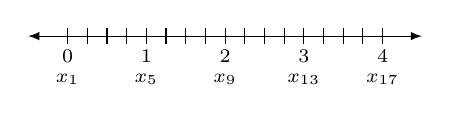
\begin{tikzpicture}[>=latex]
\draw [<->] (-.5,0) -- (4.5,0);
\foreach \x in {0,.25,...,4}
	{\draw (\x,-.1) -- (\x,.1);
	}
\draw (0,-.25) node {\scriptsize $0$};
\draw (1,-.25) node {\scriptsize $1$};
\draw (2,-.25) node {\scriptsize $2$};
\draw (3,-.25) node {\scriptsize $3$};
\draw (4,-.25) node {\scriptsize $4$};

\draw (0,-.55) node {\scriptsize $x_1$};
\draw (1,-.55) node {\scriptsize $x_5$};
\draw (2,-.55) node {\scriptsize $x_9$};
\draw (3,-.55) node {\scriptsize $x_{13}$};
\draw (4,-.55) node {\scriptsize $x_{17}$};

\end{tikzpicture}